\documentclass{article}
\usepackage[T1]{fontenc}
\usepackage{lmodern}
\usepackage{graphicx}
\usepackage{amsmath,amssymb}
\usepackage[a4paper,margin=2cm]{geometry}
\usepackage[absolute,overlay]{textpos}
\setlength{\TPHorizModule}{1mm}
\setlength{\TPVertModule}{1mm}
\usepackage[indonesian]{babel}
\usepackage{hyperref}
\setlength{\emergencystretch}{2em}
% unit: Halaman 16

\begin{document}

% === Halaman 16 (llm) ===

\vspace{213.84mm}

\begin{itemize}
    \item Contoh lain:
\end{itemize}

\vspace{10mm}

\vspace{60mm}

Sumber: http://sspai.com/26497 \hfill Rinaldi M/II4020 Kriptografi

% deskripsi: Diagram proses pertukaran kunci Diffie Hellman antara Alice dan Bob dengan keberadaan penyadap Evil Eve, menunjukkan langkah-langkah perhitungan matematika dari pembuatan nomor acak hingga penentuan Secret Key.
% bbox normalisasi: [0.1400, 0.1200, 0.8300, 0.8400]
\begin{textblock*}{144.90mm}(29.40mm,35.64mm)
\noindent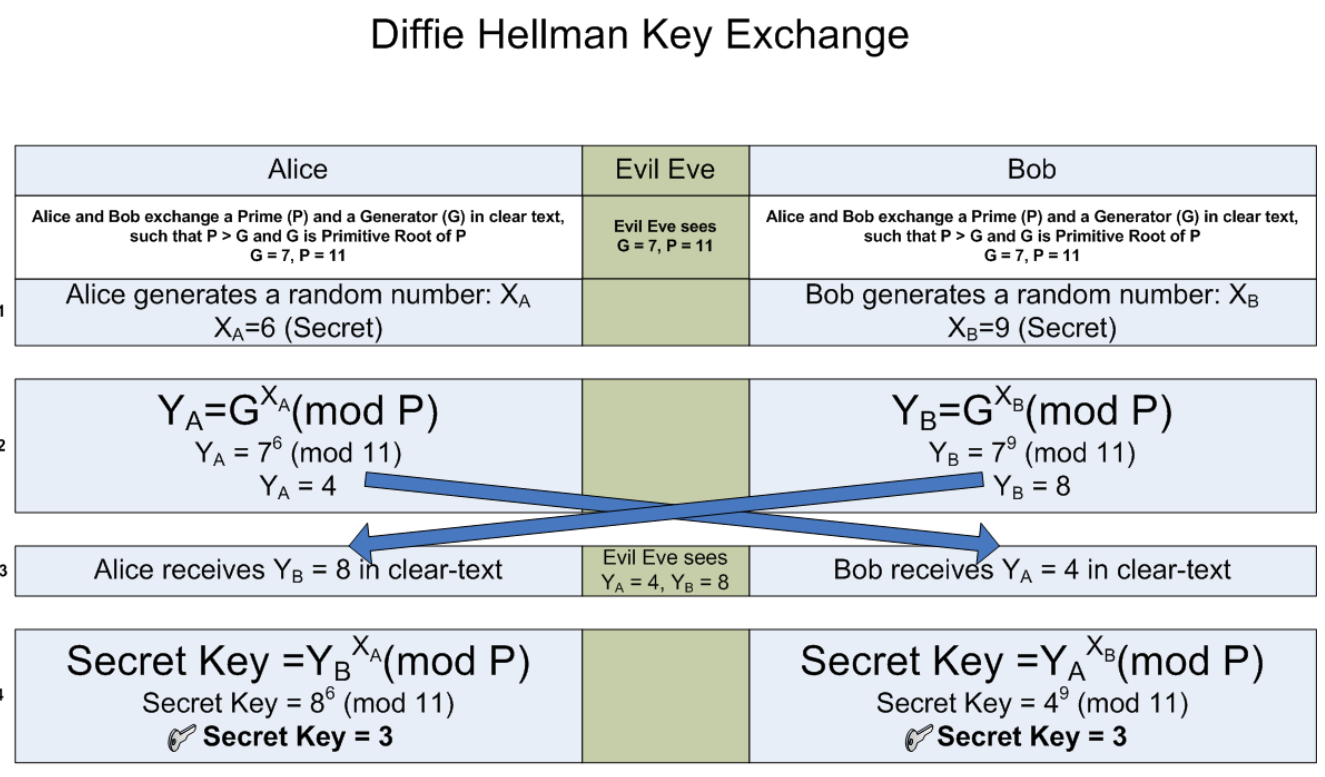
\includegraphics[width=144.90mm,height=213.84mm]{../../images/llm/page_016_img_01.png}%
\end{textblock*}

\end{document}
